\chapter{UML\cite{UML_2,Iak,Ira,Rai}}
\section{Introduccion}
UML es una notación estándar para el modelado de software para la arquitectura, diseño e implementación de software, ya sea en su estructura como en comportamiento siendo este bastante visual, al ser un lenguaje que usa diagramas este no se limita a usarse únicamente en el desarrollo de software.
UML no es un proceso de desarrollo, es decir, no describe los pasos sistemáticos a  seguir para desarrollar software. UML sólo permite documentar y especificar los elementos creados mediante un lenguaje común describiendo modelos. Es un lenguaje de propósito general para el modelado orientado a objetos, que combina notaciones provenientes desde: Modelado Orientado a Objetos, Modelado de Datos, Modelado de Componentes, Modelado de Flujos de Trabajo (Workflows).
\newpage
\newpage
\section{Historia}
El lenguaje UML comenzó a gestarse en octubre de 1994, cuando Rumbaugh se unió a la compañía Rational fundada por Booch (dos reputados investigadores en el área de metodología del software). El objetivo de ambos era unificar dos métodos que habían desarrollado: el método Booch y el OMT (Object Modelling Tool ). El primer borrador apareció en octubre de 1995. En esa misma época otro reputado investigador, Jacobson, se unió a Rational y se incluyeron ideas suyas. Estas tres personas son conocidas como los “tres amigos”. Además, este lenguaje se abrió a la colaboración de otras empresas para que aportaran sus ideas. Todas estas colaboraciones condujeron a la definición de la primera versión de UML. Figura 1: Logo de UML Se necesitaba por tanto un lenguaje no sólo para comunicar las ideas a otros desarrolladores sino también para servir de apoyo en los procesos de análisis de un problema. Con este objetivo se creo el Lenguaje Unificado de Modelado (UML: Unified Modeling Language). UML se ha convertido en ese estándar tan ansiado para representar y modelar la información con la que se trabaja en las fases de análisis y, especialmente, de diseño. 
Esta primera versión se ofreció a un grupo de trabajo para convertirlo en 1997 en un estándar del OMG (Object Management Group http://www.omg.org). Este grupo, que gestiona estándares relacionados con la tecnología orientada a objetos (metodologías, bases de datos objetuales, CORBA, etc.), propuso una serie de modificaciones y una nueva versión de UML (la 1.1), que fue adoptada por el OMG como estándar en noviembre de 1997. Desde aquella versión han habido varias revisiones que gestiona la OMG Revision Task Force. La última versión aprobada es la 1.4. En estos momentos se está desarrollando una nueva versión en la que se incluirán cambios importantes (principalmente añadir nuevos diagramas) que conducirán a la versión 2.0 planificada para fines del 2002.

\newpage

\section{Estructura}

\subsection{Elementos de UML}

\subsubsection{Elemento Estructurales}

\begin{table}[h]
	\begin{tabular}{|l|l|l|}
		\hline
		\rowcolor[HTML]{FFFFC7} 
		\multicolumn{1}{c|}{\cellcolor[HTML]{FFFFC7}Elemento} & \multicolumn{1}{c|}{\cellcolor[HTML]{FFFFC7}Definicion}&                              \multicolumn{1}{c|}{\cellcolor[HTML]{FFFFC7}Notacion} \\ \hline
		
		Caso de uso                                                 & \begin{tabular}[a]{lll}Un caso de uso representa la forma en como un Cliente\\ (Actor) opera con el sistema en desarrollo, \\además de la forma, tipo y orden en como los elementos\\ interactúan (operaciones o casos de uso).\end{tabular} & 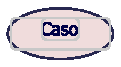
\includegraphics[width=0.1\linewidth]{imgs/casodeuso} \\ \hline
		
		Colaboracion                                                  & \begin{tabular}[c]{lll}La colaboración permite que una clase se comunique con otra\\ clase con el propósito de utilizar los métodos de esta\\ ultima para mejorar algún servicio o mantener una relación\\ lógica de dependencia.\end{tabular} & 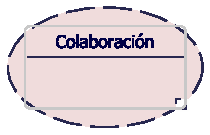
\includegraphics[width=0.1\linewidth]{imgs/colaboracion} \\ \hline			
		
		Clase                                                  & \begin{tabular}[c]{lll}Es un elemento estructural en el que se modelan atributos\\ y operaciones de un conjunto de objeto.\end{tabular} & 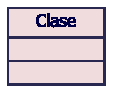
\includegraphics[width=0.1\linewidth]{imgs/clase} \\ \hline
		
		Interface                                                  & \begin{tabular}[c]{lll}Esta especifica qué se debe hacer pero no su implementación.\\ Serán las clases que implementen estas interfaces las que\\ describen la lógica del comportamiento de los métodos.\end{tabular} & 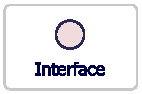
\includegraphics[width=0.1\linewidth]{imgs/interface} \\ \hline
		
		Componente                                                 & \begin{tabular}[c]{lll}Un componente, también denominado componente simple o \\atómico, es un objeto que tiene una representación gráfica, \\que se puede mostrar en la pantalla y con la que puede\\ interactuar el usuario. \end{tabular} & 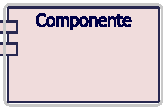
\includegraphics[width=0.1\linewidth]{imgs/componente} \\ \hline
		
		Nodo		                                                 & \begin{tabular}[c]{lll}un nodo es cada uno de los elementos de una lista enlazada\\, un árbol o un grafo en una estructura de datos.\\ Cada nodo tiene sus propias características\\ y cuenta con varios campos; al menos uno de éstos debe\\ funcionar como punto de referencia para otro nodo. \end{tabular} & 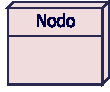
\includegraphics[width=0.1\linewidth]{imgs/nodo} \\ \hline		
		
		Artefacto                                                  & \begin{tabular}[c]{lll}En términos generales de software, un artefacto es\\ algo producido por el proceso de desarrollo de software,\\ ya sea una documentación relacionada con el software\\ o un archivo ejecutable. \end{tabular} & 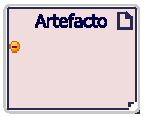
\includegraphics[width=0.1\linewidth]{imgs/artefacto} \\ \hline
	\end{tabular}
\end{table}

\newpage
\subsubsection{Elemento de Comportamiento}
\begin{center}
	\begin{table}[h]
		\begin{tabular}{|l|l|l|}
			\hline
			\rowcolor[HTML]{FFFFC7} 
			\multicolumn{1}{c|}{\cellcolor[HTML]{FFFFC7}Elemento} & \multicolumn{1}{c|}{\cellcolor[HTML]{FFFFC7}Definicion}&                              \multicolumn{1}{c|}{\cellcolor[HTML]{FFFFC7}Notacion} \\ \hline
			
			Estado	                                                   & \begin{tabular}[c]{lll}El diagrama de estado se usa para dar forma al \\comportamiento de un objeto, de una clase. Se representa\\ la secuencia de estados que un objeto de la clase tiene \\durante su vida, según las acciones que van sucediendo.\end{tabular} & 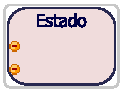
\includegraphics[width=0.1\linewidth]{imgs/estado} \\ \hline			
			
			Actividad	                                                   & \begin{tabular}[c]{lll}Básicamente se puede decir que el diagrama de actividades \\modela el flujo de actividades. Estos pueden ser procesos\\ dentro de un sistema informático, procesos de casos de uso\\ o procesos comerciales.Estas actividades pueden \\descomponerse en muchas actividades secundarias más\\ pequeñas: las acciones, que pueden llevarse a cabo \\cronológicamente. \end{tabular} & 
\includegraphics[width=0.1\linewidth]{imgs/actividad} \\ \hline
						
			Transicion                                                   & \begin{tabular}[c]{lll}Es un comportamiento que comprende un conjunto \\de mensajes intercambiados entre un conjunto de\\ objetos,\\ dentro de un contexto particular para \\alcanzar un propósito especifico.\end{tabular} & 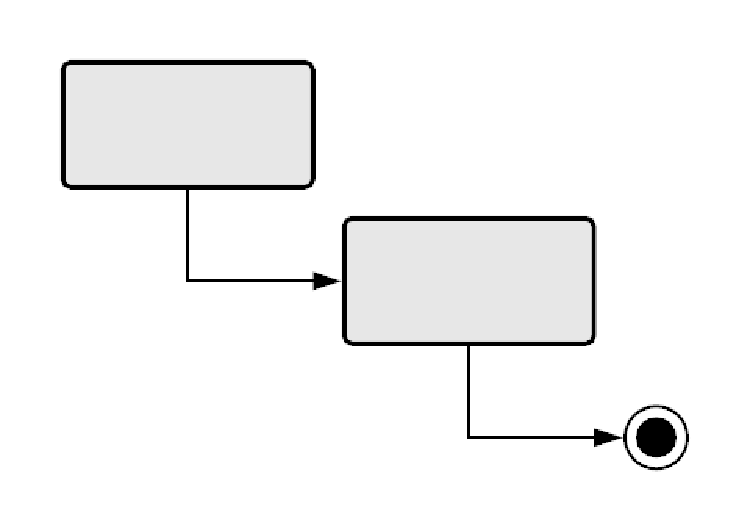
\includegraphics[width=0.1\linewidth]{imgs/transicion} \\ \hline
			

			
			
		\end{tabular}
	\end{table}	
\end{center}



\subsubsection{Elemento Agrupación}
\begin{table}[h]
	\begin{tabular}{|l|l|l|}
		\hline
		\rowcolor[HTML]{FFFFC7} 
		\multicolumn{1}{c|}{\cellcolor[HTML]{FFFFC7}Elemento} & \multicolumn{1}{c|}{\cellcolor[HTML]{FFFFC7}Definicion}                                                                                     & Notacion \\ \hline
		Sistema                                                 & \begin{tabular}[c]{lll}Es un mecanismo de propósito general para organizar\\ elementos en grupos.\\
			En estos se pueden agrupar los elementos estructurales,\\de comportamiento e incluso otros elementos de agrupación,\\
			son los elementos de agrupación básicos con los cuales\\se puede organizar un modelo UML.\end{tabular} & 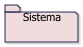
\includegraphics[width=0.12\linewidth]{imgs/paquete} \\ \hline
		
		Frame                                                & \begin{tabular}[c]{lll}\\ Similar al Sistema, usado mas en diagramas dinamicos\\ \\ \end{tabular} & 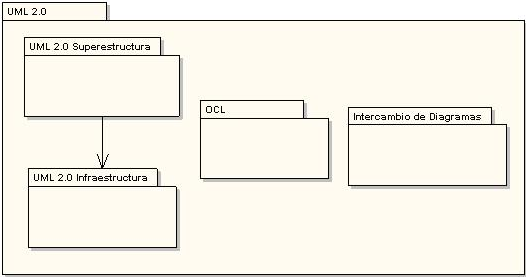
\includegraphics[width=0.1\linewidth]{imgs/frame} \\ \hline
	\end{tabular}
\end{table}

\subsubsection{Elemento Anotación}
\begin{table}[h!]
	\begin{tabular}{|l|l|l|}
		\hline
		\rowcolor[HTML]{FFFFC7} 
		\multicolumn{1}{c|}{\cellcolor[HTML]{FFFFC7}Elemento} & \multicolumn{1}{c|}{\cellcolor[HTML]{FFFFC7}Definicion}                                                                                     & Notacion \\ \hline
		Nota                                                  & \begin{tabular}[c]{lll}Son comentarios que se pueden aplicar para describir,\\ clasificar y hacer observaciones sobre cualquier \\elemento de un modelo.\\
			El tipo principal de anotación es la nota que \\simplemente es un símbolo para mostrar \\restricciones y comentarios junto a un elemento \\o un conjunto de elementos. \end{tabular} & 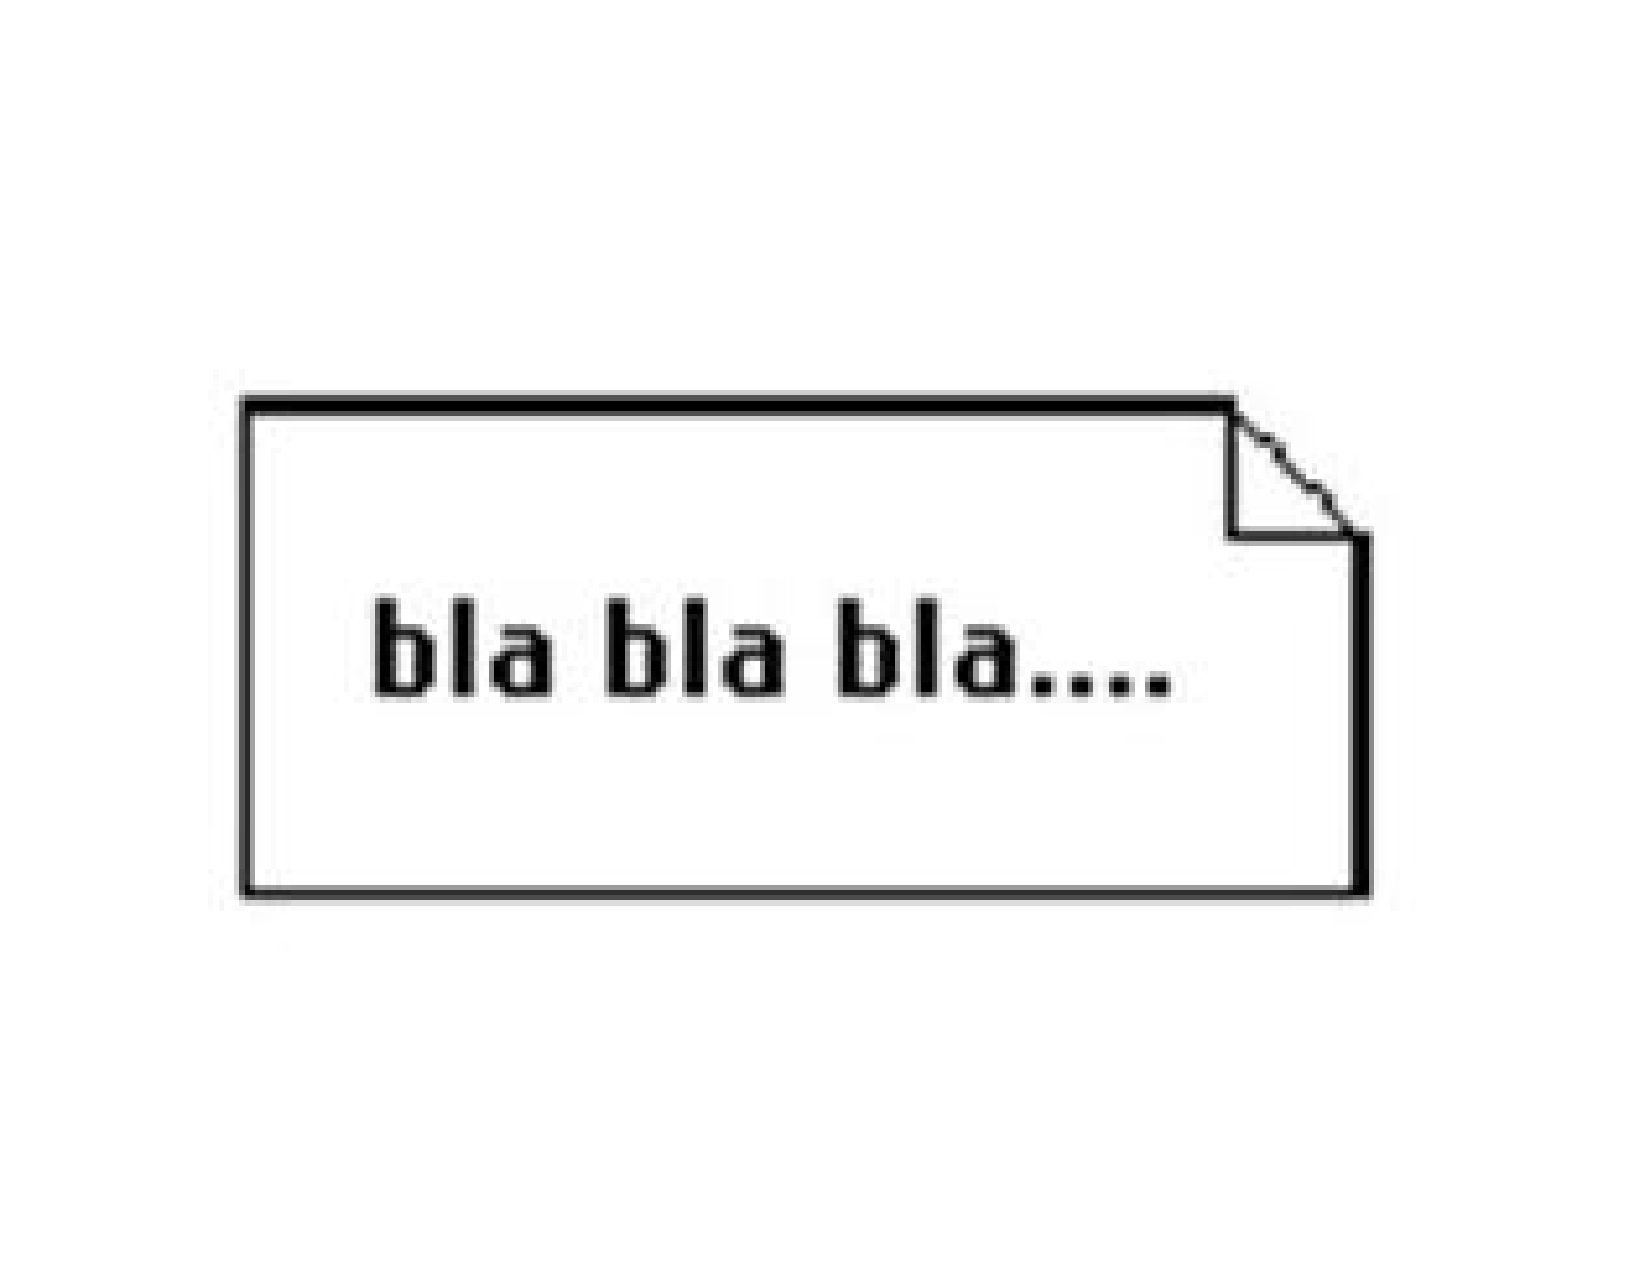
\includegraphics[width=0.15\linewidth]{imgs/nota} \\ \hline
	\end{tabular}
\end{table}


\newpage

\subsection{Relaciones de UML}

\subsubsection{Relaciones Estructurlaes}
	\begin{table}[h]
	\begin{tabular}{|l|l|l|}
\hline
\rowcolor[HTML]{FFFFC7} 
\multicolumn{1}{c|}{\cellcolor[HTML]{FFFFC7}Elemento} & \multicolumn{1}{c|}{\cellcolor[HTML]{FFFFC7}Definicion}&                              \multicolumn{1}{c|}{\cellcolor[HTML]{FFFFC7}Notacion} \\ \hline
		
		Dependencia	                                                   & \begin{tabular}[c]{lll}Es una relación de significado entre dos elementos, donde \\cualquier cambio a un elemento independiente,\\ puede afectar el significado de otro elemento dependiente. \end{tabular} & 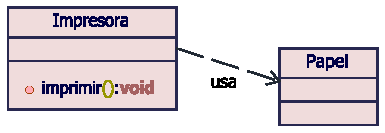
\includegraphics[width=0.27\linewidth]{imgs/dependencia} \\ \hline			
		
		Asociacion	                                                   & \begin{tabular}[c]{lll}Las asociaciones representan las relaciones más\\ generales entre clases, es decir, las relaciones con\\ menor contenido semántico. Para UML una asociación va\\ a describir un conjunto de vínculos entre las instancias \\de las clases. \end{tabular} & 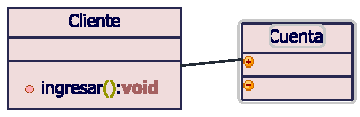
\includegraphics[width=0.27\linewidth]{imgs/asociacion} \\ \hline
		
		Agregacion                                                   & \begin{tabular}[c]{lll}Es muy similar a la relación de Asociación solo varía\\ en la multiplicidad ya que en lugar de ser una relación\\ "uno a uno" es de "uno a muchos".\end{tabular} & 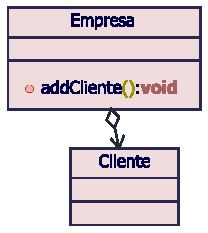
\includegraphics[width=0.3\linewidth]{imgs/agragacion} \\ \hline
		
	\end{tabular}
\end{table}	
\newpage
	\begin{table}[h]
	\begin{tabular}{|l|l|l|}
		\hline
		Composicion                                                   & \begin{tabular}[c]{lll}Aporta documentación conceptual ya que\\ es una "relación de vida", es decir, el tiempo de\\ vida de un objeto está condicionado por el\\ tiempo de vida del objeto que lo incluye.\end{tabular} & 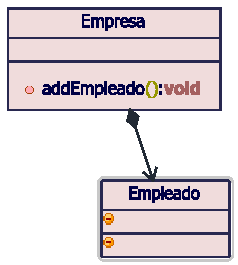
\includegraphics[width=0.25\linewidth]{imgs/composicion} \\ \hline	
	\end{tabular}
\end{table}	
\subsubsection{Relaciones de Comportamiento}
\begin{table}[h!]
	\begin{tabular}{|l|l|l|}
		\hline
		\rowcolor[HTML]{FFFFC7} 
		\multicolumn{1}{c|}{\cellcolor[HTML]{FFFFC7}Elemento} & \multicolumn{1}{c|}{\cellcolor[HTML]{FFFFC7}Definicion}&                              \multicolumn{1}{c|}{\cellcolor[HTML]{FFFFC7}Notacion} \\ \hline
		
		Generalizacion                                                  & \begin{tabular}[c]{lll}Esta hace referencia a la relación de una súper\\ clase o clase padre con una subclase o clase \\hija. La generalización significa que los objetos \\hijos se pueden emplear en cualquier clase \\donde pueda aparecer el padre, pero no a la\\ inversa. \end{tabular} & 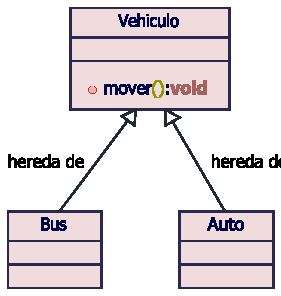
\includegraphics[width=0.3\linewidth]{imgs/generalizacion} \\ \hline
		
		Realizacion                                                  & \begin{tabular}[c]{lll}Es  una  relación  de  contrato  con  otra clase.\\  Se  la  utiliza  para  implementar  una  interfaz.  \end{tabular} & 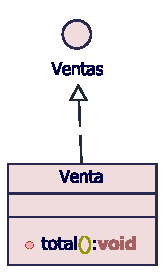
\includegraphics[width=0.25\linewidth]{imgs/realizacion} \\ \hline
	\end{tabular}
\end{table}

\newpage

\subsection{Diagramas de UML}

\subsubsection{Diagramas Estáticos (o Estructurales)}
\begin{table}[h!]
	\begin{tabular}{|l|l|l|}
		\hline
		\rowcolor[HTML]{FFFFC7} 
		\multicolumn{1}{c|}{\cellcolor[HTML]{FFFFC7}Elemento} & \multicolumn{1}{c|}{\cellcolor[HTML]{FFFFC7}Definicion}&                              \multicolumn{1}{c|}{\cellcolor[HTML]{FFFFC7}Notacion} \\ \hline
		
		Clases                                                  & \begin{tabular}[c]{lll} Describe la estructura de un sistema\\ mostrando las clases del sistema, sus\\ atributos, operaciones (o metodos), y las \\relaciones entre los objetos. \end{tabular} & 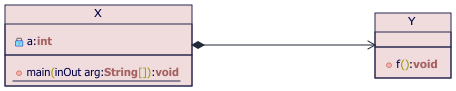
\includegraphics[width=0.32\linewidth]{imgs/clases} \\ \hline
		
		Objetos                                                  & \begin{tabular}[c]{lll} Los diagramas de objetos modelan las\\ instancias de elementos contenidos en los \\diagramas de clases.Un diagrama de objetos \\muestra un conjunto de objetos y sus \\relaciones en un momento concreto. \end{tabular} & 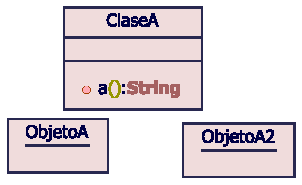
\includegraphics[width=0.32\linewidth]{imgs/objetos} \\ \hline
		
		Componentes                                                  & \begin{tabular}[c]{lll} Un diagrama de componentes representa \\cómo un sistema de software es dividido en \\componentes y muestra las dependencias\\ entre estos componentes. \end{tabular} & 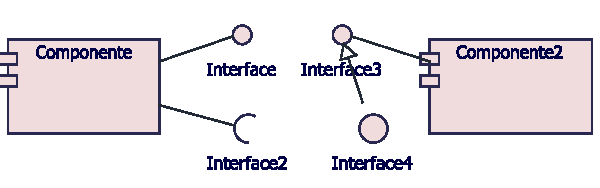
\includegraphics[width=0.32\linewidth]{imgs/componentes} \\ \hline
		
		Sistemas                                                  & \begin{tabular}[c]{lll} Muestra como un proyecto esta dividido en \\agrupaciones logicas mostrando las\\ dependencias entre esas agrupaciones. \end{tabular} & 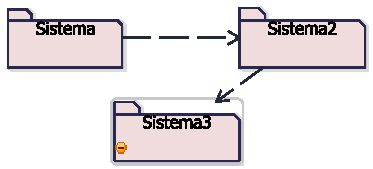
\includegraphics[width=0.32\linewidth]{imgs/sistemas} \\ \hline
		
		Estructura Compuesta                                                  & \begin{tabular}[c]{lll} Muestra la estructura interna de una \\clase y las colaboraciones que esta\\ estructura hace posibles.  \end{tabular} & 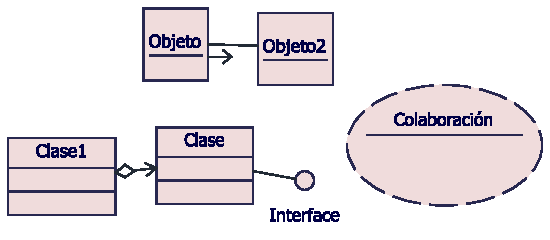
\includegraphics[width=0.35\linewidth]{imgs/estructuraCompuesta} \\ \hline
		
		
	\end{tabular}
\end{table}

\subsubsection{Diagramas dinámicos (o de Comportamiento)}
\begin{table}[h!]
	\begin{tabular}{|l|l|l|}
		\hline
		\rowcolor[HTML]{FFFFC7} 
		\multicolumn{1}{c|}{\cellcolor[HTML]{FFFFC7}Elemento} & \multicolumn{1}{c|}{\cellcolor[HTML]{FFFFC7}Definicion}&                              \multicolumn{1}{c|}{\cellcolor[HTML]{FFFFC7}Notacion} \\ \hline
		
		Casos de uso                                                 & \begin{tabular}[c]{lll} Los diagramas de caso de \\uso modelan la funcionalidad \\del sistema usando actores y \\casos de uso. \end{tabular} & 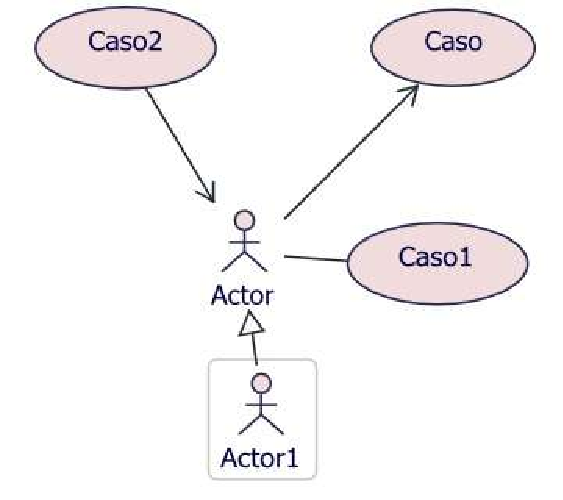
\includegraphics[width=0.25\linewidth]{imgs/casosdeuso} \\ \hline
		
		Secuencias                                                  & \begin{tabular}[c]{lll} Un diagrama de secuencia es\\un tipo de diagrama de \\interacción porque describe \\cómo (y en qué orden) un\\ grupo de objetos \\funcionan en conjunto. \end{tabular} & 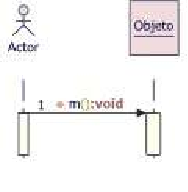
\includegraphics[width=0.25\linewidth]{imgs/secuencia} \\ \hline
		
		Comunicacion                                                  & \begin{tabular}[c]{lll} Un diagrama de comunica-\\-ción modela las interaccio-\\nes entre objetos o partes en\\ términos de mensajes en \\secuencia.  \end{tabular} & 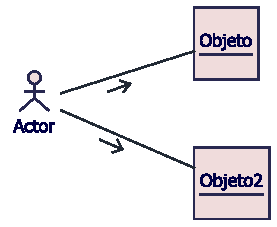
\includegraphics[width=0.25\linewidth]{imgs/comunicacion} \\ \hline
		
		Estados                                                  & \begin{tabular}[c]{lll} Es un diagrama que muestra \\transiciones entre diversos \\objetos.  \end{tabular} & 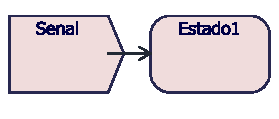
\includegraphics[width=0.25\linewidth]{imgs/estados} \\ \hline
		
		Actividades                                                  & \begin{tabular}[c]{lll} Representa los flujos de \\trabajo paso a paso de \\negocio y operacionales de \\componentes en un sistema.  \end{tabular} & 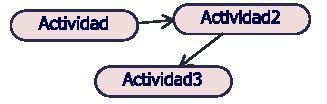
\includegraphics[width=0.35\linewidth]{imgs/actividades} \\ \hline

		Vista Conjunta de Interaccion                                                  & \begin{tabular}[c]{lll} Es una representacion grafica\\ de una interaccion, este\\ se distingue fuertemente\\ de los diagramas desecuencia \\y de comunicacion,\\ dos de los otrosdiagramas de\\ interaccion.  \end{tabular} & 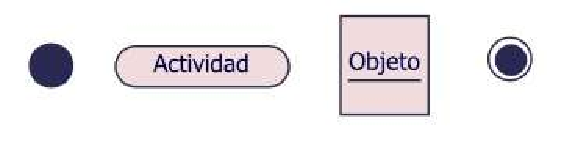
\includegraphics[width=0.35\linewidth]{imgs/vistaconjunta} \\ \hline
	\end{tabular}
\end{table}

%\begin{figure}[h]
%	\centering
%	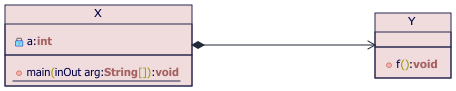
\includegraphics[width=0.7\linewidth]{imgs/clases}
%	\caption{Clases}
%\end{figure}


\newpage